Im nachfolgenden Teil des Fachberichtes wird die entwickelte Hardware des Phased Arrays näher beschrieben. Das Ziel ist es, eine möglichst modulare und skalierbare Schaltung zu entwickeln. Als Hardwareumgebung für den Mikrocontroller dient ein schon bestehendes Evaluationsboard. Das dazugehörige Layout ist frei verfügbar und vom Preis her erschwinglich. Die in diesem Projekt entwickelte Hardware ist auf der Rückseite mit Pins ausgestattet, so dass sie als Modul auf das Evaluationsboard gesteckt werden kann. Auf der Vorderseite befindet sich ein Ultraschall Phased Array und die dazugehörige Analogschaltung. Die elektronischen Komponenten sind oberflächenmontiert.


%%%%%%%%%%%%%%%%%%%%%%%%%%%%%%%%%%%%%%%%%%%%%%%%%%%%%%%%%%%%%%%%%%%%%%%%%%%%%%%%
%%%%%%%%%%%%%%%%%%%%%%%%%%%%%%%%%%%%%%%%%%%%%%%%%%%%%%%%%%%%%%%%%%%%%%%%%%%%%%%%
%%%%%%%%%%%%%%%%%%%%%%%%%%%%%%%%%%%%%%%%%%%%%%%%%%%%%%%%%%%%%%%%%%%%%%%%%%%%%%%%
\subsection{Überblick}\label{sec:ueberblick}
Die Abbildung \ref{fig:image_hardware_schema} zeigt das Gesamtsystem. Das Arduino Board stellt das Evaluationsboard dar, das Arduino Shield die in diesem Projekt entwickelte Hardware. Es ist zu sehen, dass das PWM-Modul des Mikrocontrollers über eine analoge Senderschaltung (Levelshifter) das Ultraschall Transceiver Array ansteuert und dieses wiederum die empfangenen Signale über die analoge Empfängerschaltung (Operationsverstärker und Analogschalter) auf den Analog-Digital-Konverter des Mikrocontrollers gibt. Die digitalisierten Daten werden von dort aus per DMA (direct memory access) über eine USB-Schnittstelle an das Desktop-Betriebssystem weitergeleitet.

%%%%%%%%%%%%%%%%%%%%%%%%%%%%%%%%%%%%%%%%%%%%%%%%%%%%%%%%%%%%%%%%%%%%%%%%%%%%%%%%
% pictures
\begin{figure}[htb]
\includegraphics[width=\textwidth]{graphics/image_hardware_schema.png}
\caption{Blockschaltbild des Gesamtsystems} % picture caption
\label{fig:image_hardware_schema}
\end{figure}
%
%(Abb. \ref{fig:image1})
%%%%%%%%%%%%%%%%%%%%%%%%%%%%%%%%%%%%%%%%%%%%%%%%%%%%%%%%%%%%%%%%%%%%%%%%%%%%%%%%

In Abbildung \ref{fig:image_hardware_print} ist die Hardware des Ultraschall Phased Arrays zu sehen, welche als Modul auf den Arduino Due gesteckt ist. Oben in der Mitte sind die acht Ultraschalltransceiver (1) zu sehen. Diese können sowohl zum Senden als auch zum Empfangen benutzt werden. Neben den Ultraschalltransceivern ist auf jeder Seite je ein Levelshifter (2) angebracht. Diese sind als Verstärker für das Senden zuständig. Ausserdem werden sie zum Dämpfen der Ultraschalltransceiver nach dem Sendevorgang verwendet. Direkt unterhalb der Ultraschalltransceiver befinden sich zwei Analogschalter (3), welche die empfindliche Empfängerschaltung während des Sendevorgans von den Ultraschalltransceivern und somit von der Senderschaltung trennen. Unterhalb der Analogschalter befinden sich die acht Verstärkerschaltungen (4) des Empfängerteils. Direkt unter dem linken Levelshifter ist eine Spannungsfolgerschaltung (5) zu sehen, mit welcher die Referenzspannung für die Empfängerschaltung erzeugt wird. Unten links sind die beiden Stützkondensatoren (6) für die Spannungsversorgungen von $3.3 \mathrm{V}$ und $5.0 \mathrm{V}$ zu sehen.

%%%%%%%%%%%%%%%%%%%%%%%%%%%%%%%%%%%%%%%%%%%%%%%%%%%%%%%%%%%%%%%%%%%%%%%%%%%%%%%%
% pictures
\begin{figure}[htb]
\begin{center}
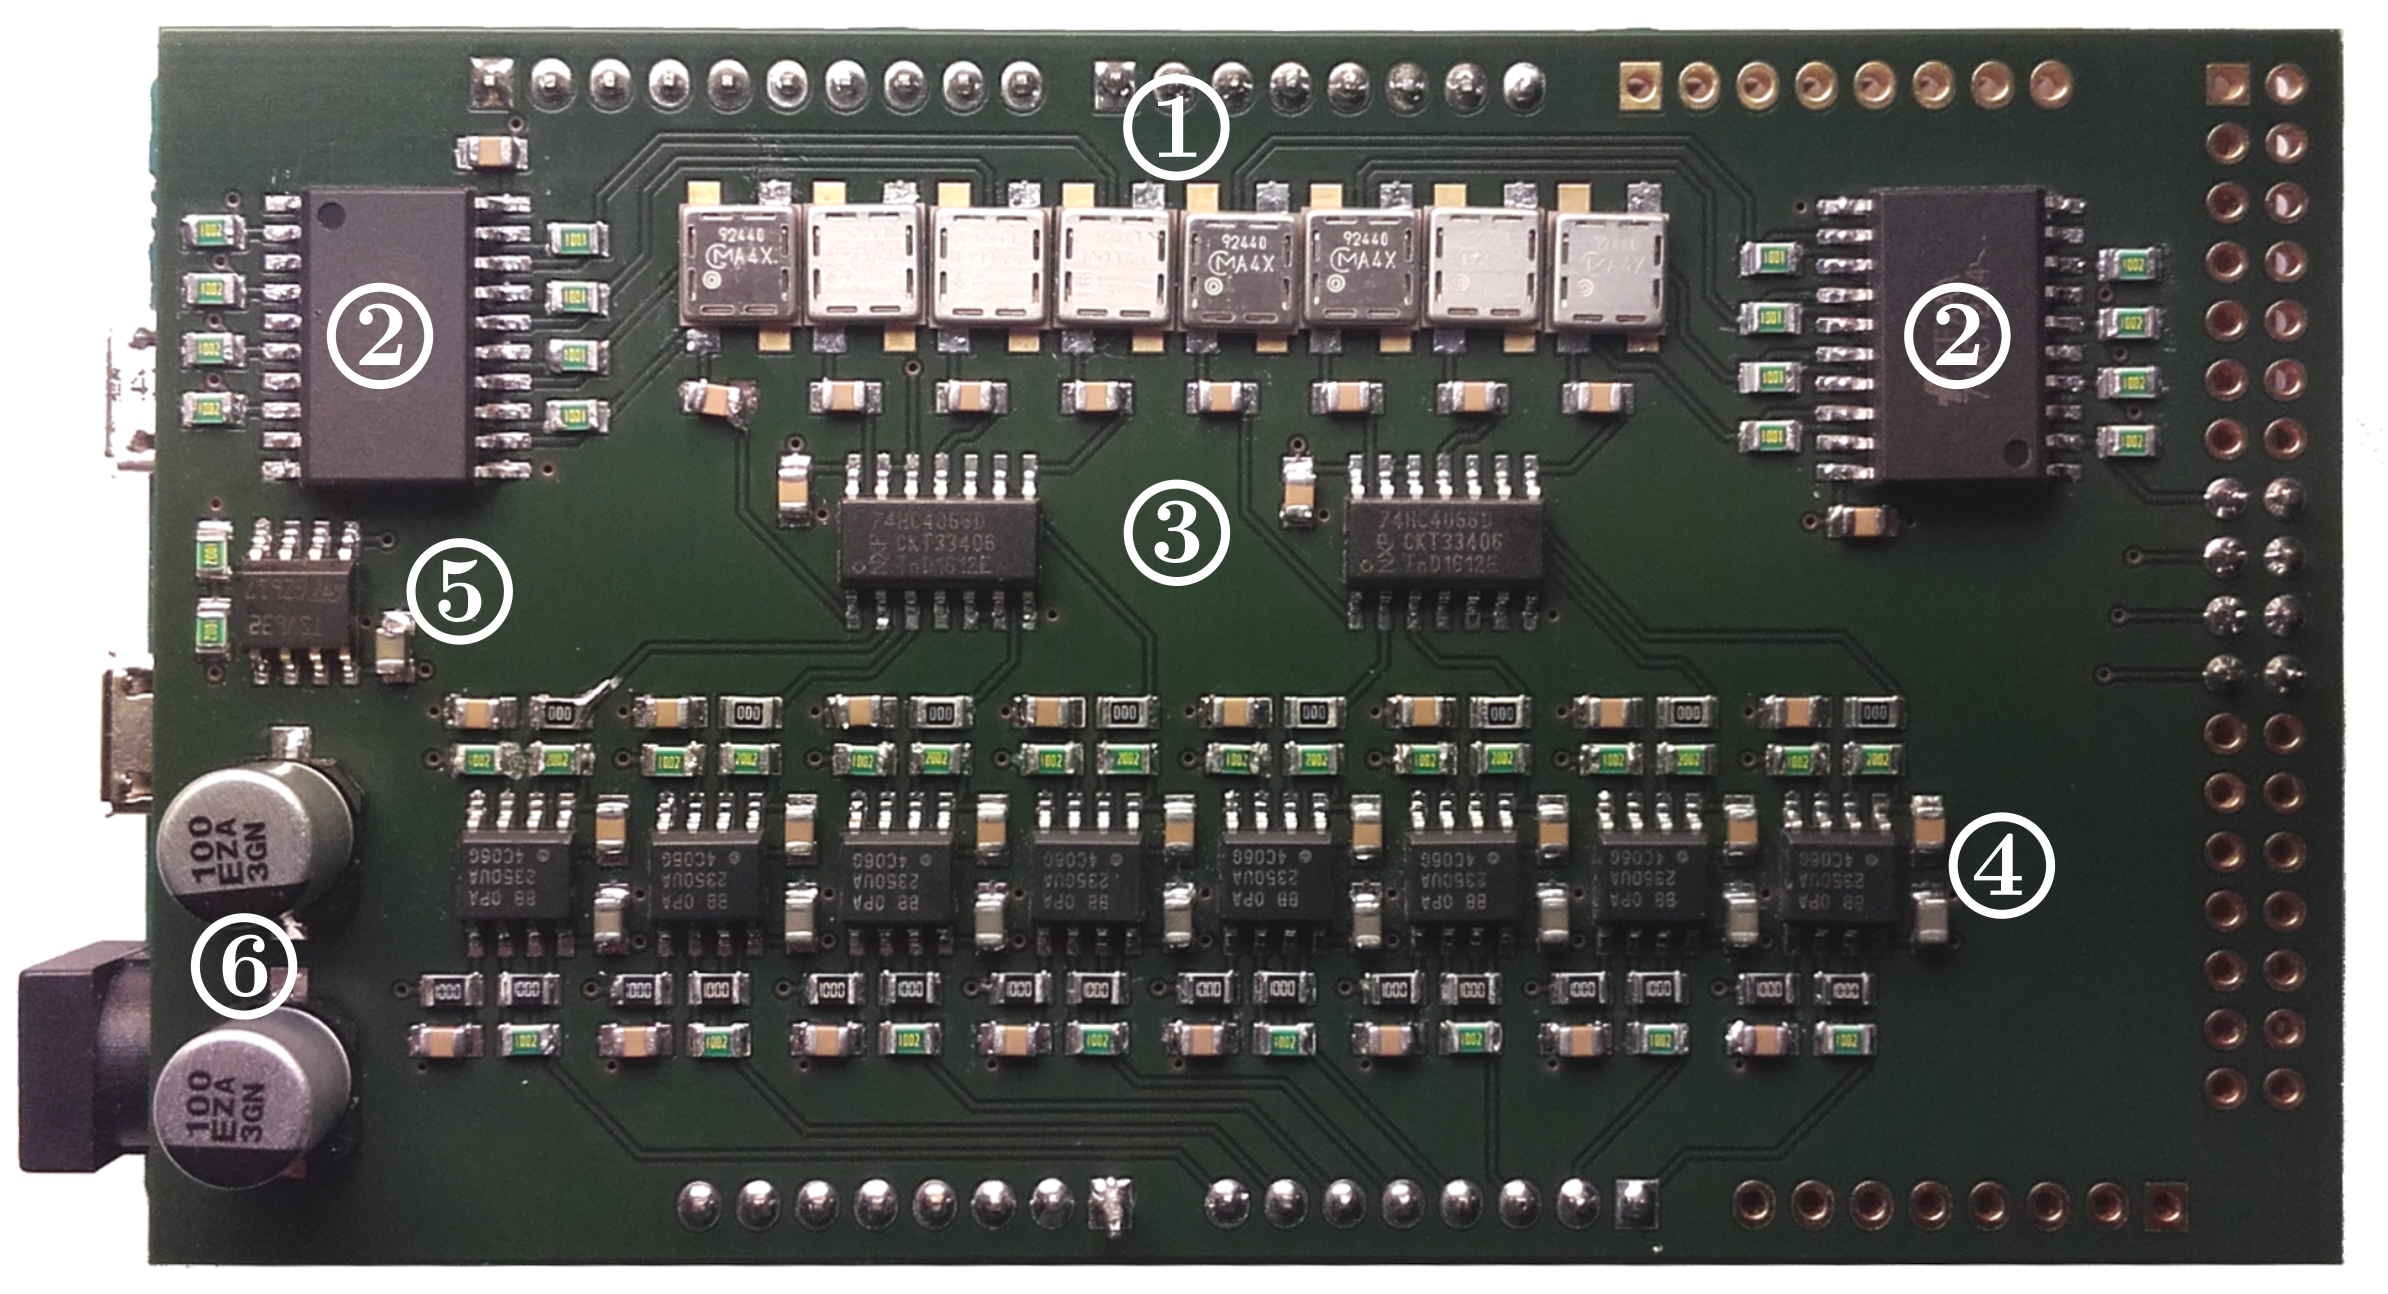
\includegraphics[width=\textwidth]{graphics/image_hardware_print.png}
\end{center}
\caption{Fertig bestückter Print} % picture caption
\label{fig:image_hardware_print}
\end{figure}
%
%(Abb. \ref{fig:image1})
%%%%%%%%%%%%%%%%%%%%%%%%%%%%%%%%%%%%%%%%%%%%%%%%%%%%%%%%%%%%%%%%%%%%%%%%%%%%%%%%


%%%%%%%%%%%%%%%%%%%%%%%%%%%%%%%%%%%%%%%%%%%%%%%%%%%%%%%%%%%%%%%%%%%%%%%%%%%%%%%%
%%%%%%%%%%%%%%%%%%%%%%%%%%%%%%%%%%%%%%%%%%%%%%%%%%%%%%%%%%%%%%%%%%%%%%%%%%%%%%%%
%%%%%%%%%%%%%%%%%%%%%%%%%%%%%%%%%%%%%%%%%%%%%%%%%%%%%%%%%%%%%%%%%%%%%%%%%%%%%%%%
\subsection{Ultraschall Phased Array}\label{sec:ultraschall_phased-array}
Das Phased Array besteht im Gegensatz zu demjenigen in Projekt 5 aus nur einer Reihe von $1$x$8$ Ultraschalltransceivern, die gleichzeitig als Sender und Empfänger dienen. Da die Ultraschalltransceiver die teuersten Komponenten des Phased Arrays sind, können dadurch die Kosten deutlich gesenkt werden (siehe Anhang \ref{sec:appendix_kosten}). Mit je einer Reihe Sender- und einer Reihe Empfängermodulen besteht bei der Vorgängerschaltung der Vorteil, dass die beiden Teilschaltungen elektronisch entkoppelt sind, und somit die empfindliche Verstärkerschaltung des Empfängers vor den hohen Spannungen der Sendeschaltung geschützt ist. Jedoch ergeben sich starke akustische Kopplungen zwischen Sende- und Empfängermodulen. Dies ist genauso unerwünscht wie elektronische Koppelung, da dadurch der Ausschwingvorgang sehr lange dauert und die minimal messbare Distanz grösser wird.

Ursprünglich geplant war nur eine Reihe von fünf Ultraschalltransceivern. Aufgrund der Berechnungen im Kapitel \ref{sec:phased_array_schallquellen}, welche in der Abbildung \ref{fig:plot_grundlagen_sharpness_factor_calc_1} dargestellt sind, ist ersichtlich, dass bereits mit acht Schallquellen eine deutlich schmalere Hauptkeule in der Richtcharakteristik erzeugt werden kann.

Das Phased Array soll in Räumen eingesetzt werden. Daher werden Ultraschalltransceiver benötigt, die in Luft eine möglichst geringe Dämpfung aufweisen. Handelsübliche Ultraschallsender und Empfänger für diesen Anwendungsbereich arbeiten bei Frequenzen von ca. $30 \mathrm{kHz} - 50 \mathrm{kHz}$. Diese liegen einerseits deutlich ausserhalb des hörbaren Bereichs, andererseits sind sie noch genügend tief, um eine breite Abstrahlcharakteristik zu erzeugen. Bei höheren Frequenzen nimmt die Richtwirkung der einzelnen Module aufgrund der grösseren Dimensionen im Verhältnis zur Wellenlänge tendenziell zu, was für ein Phased Array unerwünscht ist.

Wie aus dem Kapitel \ref{sec:phased_array_schallquellen}, Abbildung \ref{fig:plot_grundlagen_characteristic_calc_1} hervorgeht, entstehen starke Nebenkeulen in der Richtcharakteristik, sobald der Abstand der Ultraschalltransceiver grösser als eine Wellenlänge wird. Die meisten im Handel erhältlichen Ultraschalltransceiver kommen daher nicht infrage, da ihre Abmessungen zu gross sind. Für das Phased Array werden die kleinsten günstig erhältlichen Ultraschalltransceiver des Typs ''Murata MA40H1S-R'' verwendet, die im Abstand von $5.4 \mathrm{mm}$ montiert werden können und eine Mittenfrequenz von $40 \mathrm{kHz}$ aufweisen. Dies entspricht einer Wellenlänge von $8.5 \mathrm{mm}$, womit der Abstand zwischen den Modulen $d = 0.635 \mathrm{\lambda}$ beträgt. In Abbildung \ref{fig:plot_hardware_characteristic_calc} ist die berechnete, theoretisch erreichbare Richtcharakteristik ohne Amplitudenbelegung für vier verschiedene Sendewinkel dargestellt.

%%%%%%%%%%%%%%%%%%%%%%%%%%%%%%%%%%%%%%%%%%%%%%%%%%%%%%%%%%%%%%%%%%%%%%%%%%%%%%%%
% pictures
\begin{figure}[htb]
\begin{center}
\includegraphics[width=\textwidth]{graphics/plot_hardware_characteristic_calc.png}
\end{center}
\caption{Richtcharakteristik mit $N = 8$ Elementen, im Abstand von $d = 0.635 \mathrm{\lambda}$} % picture caption
\label{fig:plot_hardware_characteristic_calc}
\end{figure}
%
%(Abb. \ref{fig:image1})
%%%%%%%%%%%%%%%%%%%%%%%%%%%%%%%%%%%%%%%%%%%%%%%%%%%%%%%%%%%%%%%%%%%%%%%%%%%%%%%%



\clearpage
%%%%%%%%%%%%%%%%%%%%%%%%%%%%%%%%%%%%%%%%%%%%%%%%%%%%%%%%%%%%%%%%%%%%%%%%%%%%%%%%
%%%%%%%%%%%%%%%%%%%%%%%%%%%%%%%%%%%%%%%%%%%%%%%%%%%%%%%%%%%%%%%%%%%%%%%%%%%%%%%%
%%%%%%%%%%%%%%%%%%%%%%%%%%%%%%%%%%%%%%%%%%%%%%%%%%%%%%%%%%%%%%%%%%%%%%%%%%%%%%%%
\subsection{Analogschaltung zum Phased Array}\label{sec:analogschaltung_zum_phased_array}
Für die Ansteuerung des Ultraschall Phased Arrays wird eine Analogschaltung benötigt, da einerseits die Sendesignale verstärkt werden müssen und andererseits die empfangenen Signale zu schwach sind, um sie ohne Verstärkung zu digitalisieren. Es werden also zwei unterschiedliche Verstärkerschaltungen benötigt, welche nachfolgend als Senderschaltung und Empfängerschaltung bezeichnet werden. Zur Empfängerschaltung gehört ausserdem noch die Teilschaltung, welche die Empfangsverstärker zu deren Schutz während des Sendens von den Ultraschall\-trans\-ceivern trennt. Zur Sendeschaltung gehört zusätzlich eine Schaltung, mit der die Ultraschall\-trans\-ceiver gedämpft werden können, um damit die Ausschwingzeit zu verkürzen. Dadurch reduziert sich auch die minimal messbare Distanz. Nachfolgend werden diese Schaltungen näher erläutert.

\subsubsection{Empfängerschaltung}\label{sec:empfaengerschaltung}
Aufgabe der Empfängerschaltung ist es, die von den Ultraschallsensoren empfangenen Signale zu verstärken und an den Analog-Digital-Konverter des Mikrocontrollers weiterzuleiten. Ausserdem muss die Verstärkerschaltung aufgrund ihrer Empfindlichkeit während des Sendevorgangs von den Ultraschalltransceivern getrennt werden. Dafür werden zwei Analogschalter mit je vier Kanälen verwendet. Abbildung \ref{fig:image_hardware_opamp} zeigt die Empfängerschaltung und einen Teil der Senderschaltung für einen Kanal. Die anderen sieben Kanäle sind identisch aufgebaut. Der Analogschalter (U3A) kann nur Spannungen zwischen $0.0 \mathrm{V}$ und $5.0 \mathrm{V}$ schalten, da er keine negative Versorgungsspannung aufweist. Da nun aber der Ultraschalltransceiver (X1) als Bezugspotential $0.0 \mathrm{V}$ hat und während des Empfangens auch in den negativen Bereich schwingt, ist zwischen Ultraschalltransceiver und Analogschalter ein Kondensator (C15) zum Entkoppeln eingebaut. Die andere Seite des Analogschalters hängt über die Operationsverstärkerschaltung auf dem Potential der Referenzspannung V\_REF von $1.65 \mathrm{V}$. Über das Signal REC\_EN (receiver enable) wird der Analogschalter direkt vom Mikrocontroller angesteuert.

Wie in der Abbildung \ref{fig:image_hardware_opamp} ebenfalls zu sehen ist, werden für die Verstärkung zwei kaskadierte Operationsverstärker verwendet. Wichtig bei der Auswahl der Operationsversärker ist, dass diese bis zu einer Frequenz von $50 \mathrm{kHz}$ eine genügend hohe Verstärkung im Bereich von 100 bis 200 aufweisen. Da die Piezoelemente der Ultraschalltransceiver selber schon sehr schmalbandige Filter darstellen, ist eine weitere Bandpassfilterung vor der Unterabtastung unnötig. Es ist aber darauf zu achten, dass die Verstärkerschaltung möglichst rauscharm ist, weil sich bei einer Unterabtastung der Signale das Rauschen stark auf die Signalqualität auswirkt.

Die Referenzspannung V\_REF von $1.65 \mathrm{V}$ wird für alle acht Kanäle über eine Spannungsfolgerschaltung erzeugt und über ein RC-Tiefpassfilter (R18/C23 und R42/C39) an den nichtinvertierenden Eingang der Operationsverstärker gelegt. Das Tiefpassfilter dient dazu, allfällige hochfrequente Störungen direkt vor dem Operationsverstärker zu dämpfen. Die Grenzfrequenz für den ersten Operationsverstärker wurde um den Faktor 100 kleiner (bei ca. $150 \mathrm{Hz}$) gewählt als für den zweiten, da bei jenem wesentlich kleinere und störanfälligere Signale anliegen.

Die kompletten Empfänger- und Senderschaltungen kommen ohne negative Spannung aus. Die Operationsverstärker werden zwischen $0.0 \mathrm{V}$ und $3.3 \mathrm{V}$ betrieben, weshalb ein Single-Supply Rail-to-Rail Operationsversärker eingesetzt wird. Der Operationsverstärker OPA2350UA weist ein genügend grosses Gain-bandwidth Product und eine ausreichende Slew-Rate auf, um bei mindestens $50 \mathrm{kHz}$ eine Verstärkung von über $200$ zu erzielen, und erfüllt damit die nötigen Anforderungen.

Da eine Verstärkung um den Faktor $200$ insgesamt zu klein ist, sind pro Ultraschallempfänger jeweils zwei Operationsverstärker kaskadiert. Die Verstärkung des ersten Operationsverstärkers (U5A) hängt neben dem Rückkopplungswiderstand ($\mathrm{R33} = 20 \mathrm{k \Omega}$) von der Impedanz des Piezoelements ($\mathrm{Z_{X1}} \approx 1000 \mathrm{\Omega}$), vom Schaltwiderstand des Analogschalters ($\mathrm{R_{U3A}} \approx 85 \mathrm{\Omega}$) und vom Vorwiderstand ($\mathrm{R17} = 0 \mathrm{\Omega}$) ab. Die Verstärkung beträgt somit ungefähr $18.4$, kann aber leicht variieren, weil weder der Schaltwiderstand des Analogschalters noch die Impedanz des Piezoelements ganz genau spezifiziert sind. Die Verstärkung des zweiten Operationsverstärkers beträgt $\mathrm{R57} / \mathrm{R41} = 10 \mathrm{k \Omega} / 100 \mathrm{\Omega} = 100$. Insgesamt beträgt die Verstärkung also etwa $1840$.

%%%%%%%%%%%%%%%%%%%%%%%%%%%%%%%%%%%%%%%%%%%%%%%%%%%%%%%%%%%%%%%%%%%%%%%%%%%%%%%%
% pictures
\begin{figure}[htb]
\begin{center}
\includegraphics[width=\textwidth]{graphics/image_hardware_opamp.png}
\end{center}
\caption{Schema der Operationsverstärkerschaltung} % picture caption
\label{fig:image_hardware_opamp}
\end{figure}
%
%(Abb. \ref{fig:image1})
%%%%%%%%%%%%%%%%%%%%%%%%%%%%%%%%%%%%%%%%%%%%%%%%%%%%%%%%%%%%%%%%%%%%%%%%%%%%%%%%

\subsubsection{Senderschaltung}\label{sec:senderschaltung}
Die Senderschaltung hat die Aufgabe, den Piezokristall des Ultraschalltransceivers mit einem Rechtecksignal von $0.0 - 5.0 \mathrm{V}$ und einer Frequenz von $40 \mathrm{kHz}$ in Schwingung zu versetzen. Dadurch wird ein akustischer Ton derselben Frequenz erzeugt. Um dies zu realisieren, werden zwei Levelshifter des Typs 74ACT244 verwendet, welche die Ausgangsspannung des Mikrocontrollers von $3.3 \mathrm{V}$ auf $5.0 \mathrm{V}$ erhöhen. Die Levelshifter werden dazu vom Mikrocontroller mit einem pulsweitenmodulierten Signal von $40 \mathrm{kHz}$ angesteuert. Da während des Empfangsvorgangs die Levelshifter von den Ultraschalltransceivern getrennt werden müssen, um die Messung der empfangenen Signale nicht zu beeinflussen, müssen sie unmittelbar nach dem Senden auf ''high impedance'' geschaltet werden. Aus diesem Grund werden Tristate-Levelshifter verwendet. Auch diese Steuerung erfolgt direkt durch den Mikrocontroller. Von jedem Levelshifter werden nur je vier von acht verfügbaren Kanälen für die Verstärkung des Sendesignals verwendet. Die anderen vier Kanäle werden zum Dämpfen der Ultraschalltransceiver direkt nach dem Senden benutzt. Die Ultraschalltransceiver haben bei $40 \mathrm{kHz}$ eine Impedanz von ungefähr $1 \mathrm{k \Omega}$. Daher wird durch den Levelshifter pro Kanal ein Widerstand von $1 \mathrm{k \Omega}$ parallel zum Ultraschalltransceiver gegen Ground geschaltet, um mittels Leistungsanpassung möglichst viel Energie aus dem Schwingkreis im Widerstand zu ''verheizen''. Die Funktionsweise dieser Schaltung wurde vor dem Redesign der Hardware mit einer Testschaltung an einem einzelnen Kanal mit Erfolg getestet. Abbildung \ref{fig:image_hardware_opamp} im Kapitel \ref{sec:empfaengerschaltung} zeigt den Kanal $0$ der Sende- und Empfangsschaltung. Links im Bild sind die beiden vom Levelshifter kommenden tristate Signale ''V\_PWM\_0'' und ''GND\_SW\_0'' (ground switch) zu sehen. Das erste ist das PWM-Signal zum Anregen des Piezos, über das zweite wird der Widerstand zugeschaltet.



%%%%%%%%%%%%%%%%%%%%%%%%%%%%%%%%%%%%%%%%%%%%%%%%%%%%%%%%%%%%%%%%%%%%%%%%%%%%%%%%
%%%%%%%%%%%%%%%%%%%%%%%%%%%%%%%%%%%%%%%%%%%%%%%%%%%%%%%%%%%%%%%%%%%%%%%%%%%%%%%%
%%%%%%%%%%%%%%%%%%%%%%%%%%%%%%%%%%%%%%%%%%%%%%%%%%%%%%%%%%%%%%%%%%%%%%%%%%%%%%%%
\subsection{ADC und Mikrocontroller}\label{sec:adc_und_mikrocontroller}
Für die Ansteuerung eines 1x$N$ Arrays werden auf dem Mikrocontroller $N$ ADC-Kanäle und $N$ PWM-Kanäle benötigt. Für das in diesem Projekt entwickelte Phased Array wird $N = 8$  gewählt. Gemäss den Simulationen (siehe Abbildungen \ref{fig:image_grundlagen_sim_0_degrees}, \ref{fig:image_grundlagen_sim_10_degrees} und \ref{fig:image_grundlagen_sim_20_degrees} im Kapitel \ref{sec:simulationen}) und den Berechnungen (siehe Abbildung \ref{fig:plot_hardware_characteristic_calc} im Kapitel \ref{sec:ultraschall_phased-array}) kann damit eine genügend hohe Richtwirkung erzeugt werden. Auch die anfallende Datenmenge des Analog-Digital-Konverters kann problemlos per USB gesendet und auch auf einem leistungsschwachen Desktop PC verarbeitet werden. Der ADC des Mikrocontrollers muss eine genügend hohe Abtastrate aufweisen, um die Ultraschallsignale zu empfangen. Bei einer Ultraschallfrequenz von maximal $50 \mathrm{kHz}$ und acht Kanälen (Multiplexing) ergibt sich laut dem Abtasttheorem nach Nyquist-Shannon eine Abtastfrequenz von minimal $0.8 \mathrm{MHz}$. Durch Unterabtastung lässt sich aufgrund der schmalbandigen Signale diese Anforderung aber umgehen (siehe Kapitel \ref{sec:abtasttheorem}). Um die anfallenden Datenmengen vom Mikrocontroller auf das weiterverarbeitende System (Desktop-Betriebssystem) zu übertragen, ist eine USB 2.0 Highspeed Schnittstelle mit Direct Memory Access (DMA) von Vorteil.

Ein verbreiteter Mikrocontroller, der all diese Anforderungen erfüllt, ist der SAM3X8E von Atmel. Er hat $16$ ADC-Kanäle, $16$ PWM-Kanäle, von denen aber nicht alle ohne weiteres verfügbar sind, sowie eine USB-Schnittstelle. Die Samplingfrequenz des ADC beträgt $1 \mathrm{MHz}$ (Multiplexing über alle $16$ Kanäle). Dies ist ausreichend, wenn mit Unterabtastung gearbeitet wird. Ausschlaggebend bei der Unterabtastung ist dabei auch die Sample-and-Hold-Zeit, welche bei einer Abtastrate von $1 \mathrm{MHz}$ ausreicht. Ebenfalls weist der SAM3X8E einen DMA-Controller der einerseits mit dem ADC und andererseits mit der USB-Schnittstelle zusammen verwendet werden kann.

Für dieses Projekt wird ein Arduino DUE Board eingesetzt, da es den Mikrocontroller SAM3X8E enthält, welcher alle gestellten Anforderungen erfüllt. Das Arduino DUE Board hat desweiteren den Vorteil, dass es einfach erhältlich ist und das Projekt daher relativ einfach nachgebaut werden kann. Es muss dadurch keine Zeit mit dem Aufbau eines ''eigenen'' Mikrocontrollerboards aufgewendet werden.



%%%%%%%%%%%%%%%%%%%%%%%%%%%%%%%%%%%%%%%%%%%%%%%%%%%%%%%%%%%%%%%%%%%%%%%%%%%%%%%%
%%%%%%%%%%%%%%%%%%%%%%%%%%%%%%%%%%%%%%%%%%%%%%%%%%%%%%%%%%%%%%%%%%%%%%%%%%%%%%%%
%%%%%%%%%%%%%%%%%%%%%%%%%%%%%%%%%%%%%%%%%%%%%%%%%%%%%%%%%%%%%%%%%%%%%%%%%%%%%%%%
\subsection{PCB Design}\label{sec:pcb_design}
Nachfolgend werden die wichtigsten Kriterien aufgezählt, nach denen die Leiterplatte für dieses Projekt entwickelt ist. Um Störungen möglichst gut vorzubeugen, wird ein vierlagiger Print entwickelt, was zwar teurer ist als ein zweilagiger, aber einige Vorteile bezüglich der elektromagnetischen Verträglichkeit hat. Die Bilder der einzelnen Printlayer und das komplette Schema befinden sich im Anhang \ref{sec:appendix_schema}.

Der unterste Layer ist ein Groundlayer und weist keine Signalleitungen auf. Vom Arduino DUE stammende hochfrequente induktive Störungen werden dadurch bestmöglich abgeblockt.

Der nächste Layer enthält die beiden Spannungsversorgungen von $3.3 \mathrm{V}$ und $5.0 \mathrm{V}$. Daneben verlaufen noch die digitalen Signalleitungen zum Einschalten der Analogschalter und der Levelshifter.

Der dritte Layer liegt auf dem Potential der Referenzspannung für die Operationsverstärkerschaltung des Empfängerteils. Daneben werden aussen am Rand die Signalleitungen zur Ansteuerung der Levelshifter geführt. Es ist darauf zu achten, dass keine Signalleitungen zwischen der Spannungsfolgerschaltung und den einzelnen Operationsverstärkern liegen. Die grossflächige Ausführung des Layers wirkt wie schon der Groundlayer abschirmend gegen hochfrequente induktive Kopplungen von unten.

Der oberste Layer enthält alle analogen Signalleitungen, welche sehr empfindlich sind. Alle nicht benutzten Flächen sind mit Ground ausgegossen. Bei der Führung der Signalleitungen ist darauf zu achten, dass zwischen den Leiterbahnen immer ein genügend grosser Abstand vorhanden ist, um Übersprechen zu verhindern. Für alle analogen Signale wird jeweils der kürzestmögliche Weg gewählt. Digitale Signale werden nur aussen am Rand des Layers, und niemals zu nahe bei analogen Signalen geführt.
